\subsection{Stabilizer Configuration}
Several different types of aircraft tails exist.  For the purpose of SAM Mk I, a conventional tail is recommended due to fabrication simplification and adequate stability.  A trade study was conducted to observe the difference between a high T-tail and conventional, and ruled in favor of conventional due to stability.
\begin{table}[!h]
    \centering
    \caption{Stabilizer Dimensions}
    \begin{tabular}{|c||c|c|c|} \toprule
        \textbf{Description} & {\textbf{Horizontal Stabilizer}} & 
        {\textbf{Vertical Stabilizer}} & \textbf{Units}\\ \hline \hline
        AR & 4.5 & 1.5 & $\sim$ \\ \hline
        b (\textit{span}) & 67 & 27 & ft \\ \hline 
        $s_{\text{wing}}$ (\textit{area}) & 1,000 & 500 & ft$^2$ \\ \hline
        c/4 Sweep & 35 & 35 & degree \\ \hline
        $\lambda$ & 0.35 & 0.35 & $\sim$ \\ \hline
        Chord Root & 265.01 & 324.58 & in \\ \hline
        Chord Tip & 92.76 & 113.60 & in \\ \hline   
        Mean Aerodynamic Chord & 192.71 & 236.02 & in \\ \bottomrule
    \end{tabular}
    \label{tab:stabsizing}
\end{table}

Both the horizontal and vertical stabilizer are initially sized per Raymer's recommended 25\% and 12.5\% of $S_{wing}$.\cite{raymer}  Location of the stabilizers, as notated as the distance between the $\text{MAC}_{\text{wing}}$ and $\text{MAC}_{\text{stabilizers}}$.

\subsubsection{Horizontal Stabilizer}
SAM Mk I uses a standard tail configuration.  The horizontal stabilizer is initially sized to be 25\% of $S_{wing}$.  The dimensions of the horizontal stabilizer may be seen in Figure \ref{fig:htailstab}.  This provides a starting point from which to begin stability analysis.  Use of an inverted NASA SC(2)-0412 airfoil for the horizontal stabilizer is proposed to provide a counter moment to the lifting effects of the wing.
\begin{figure}[!h]
    \centering
    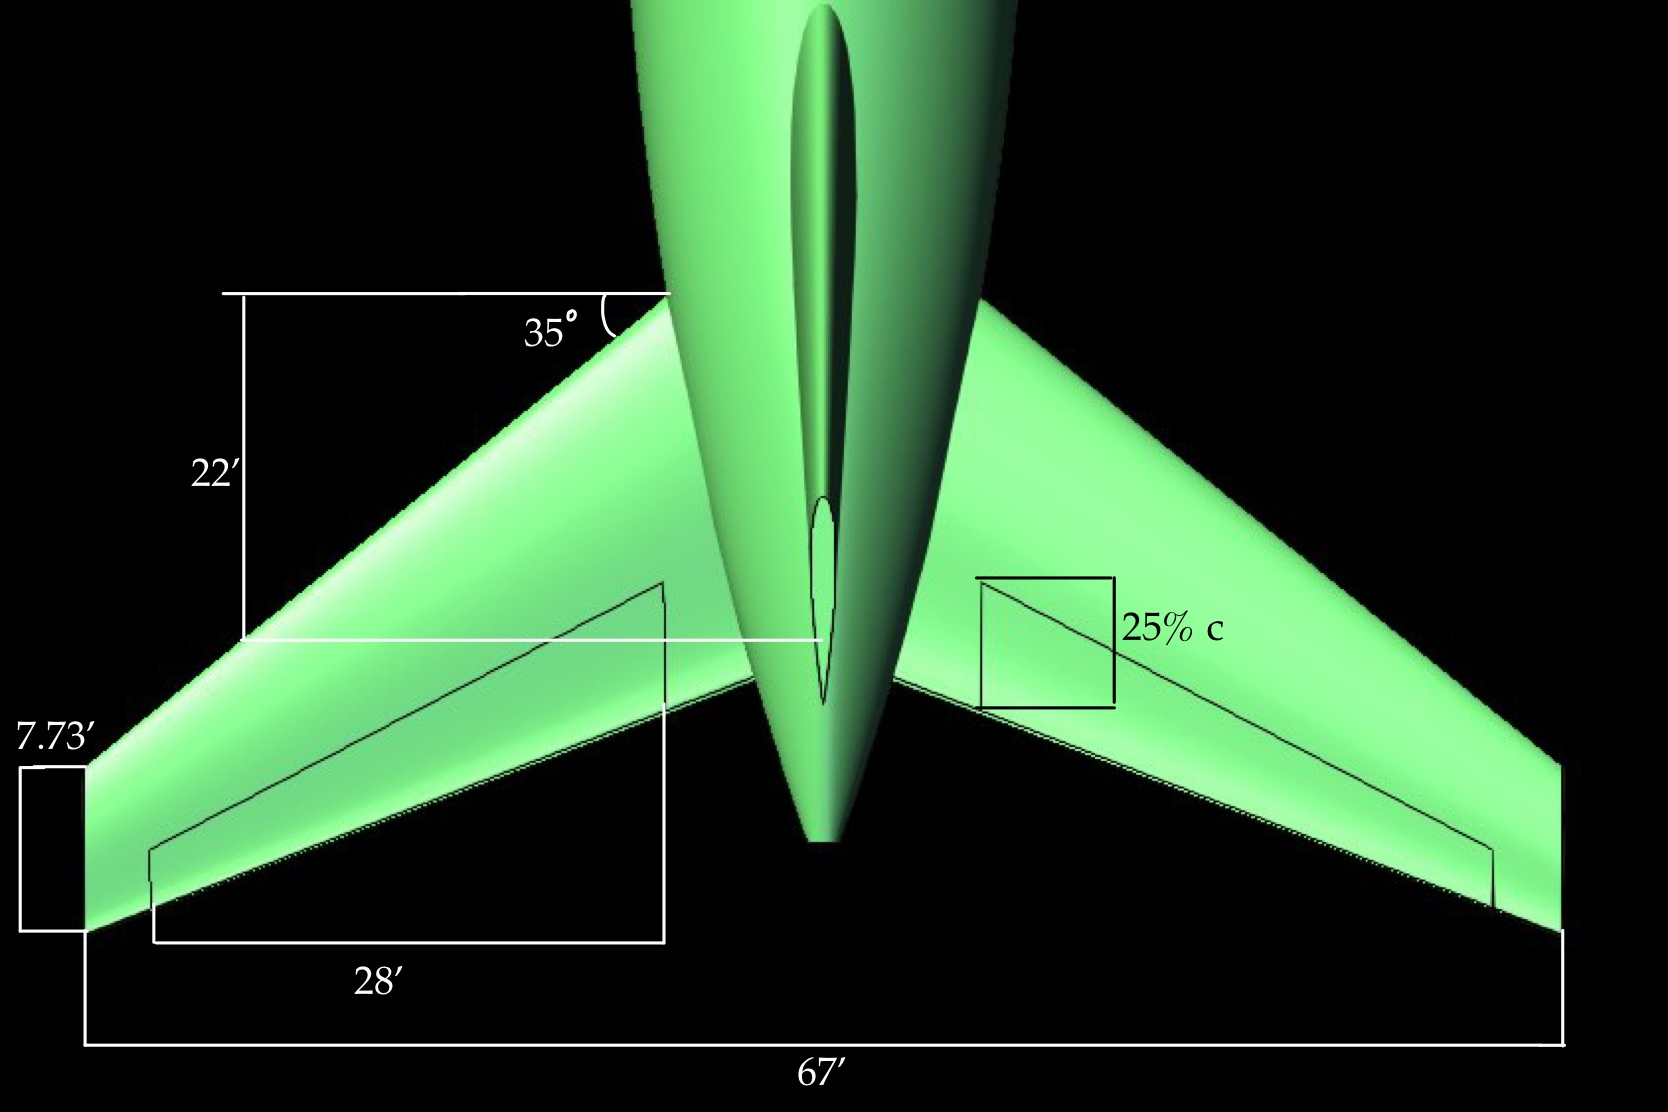
\includegraphics[width=0.75\textwidth]{Photos/stab/htail.jpg}
    \caption{Horizontal Stabilizer Top View}
    \label{fig:htailstab}
\end{figure}

\subsubsection{Vertical Stabilizer}
The vertical stabilizer is sized to be approximately 12.5\% of $S_{wing}$.  Additional attention must be directed at the vertical stabilizer to ensure directional stability.  The vertical stabilizer may be seen in Figure \ref{fig:vtailstab}.  A symmetrical airfoil is desired for the vertical stabilizer to improve the directional stability by counteracting any yaw-moments.  Due to its thin profile and symmetrical form factor, the NACA 0012 is selected for the vertical tail.  Yaw-directional trim tabs are located on the aft 5\% chordwise trailing edge of the vertical tail to provide a trim factor.

\begin{figure}[!h]
    \centering
    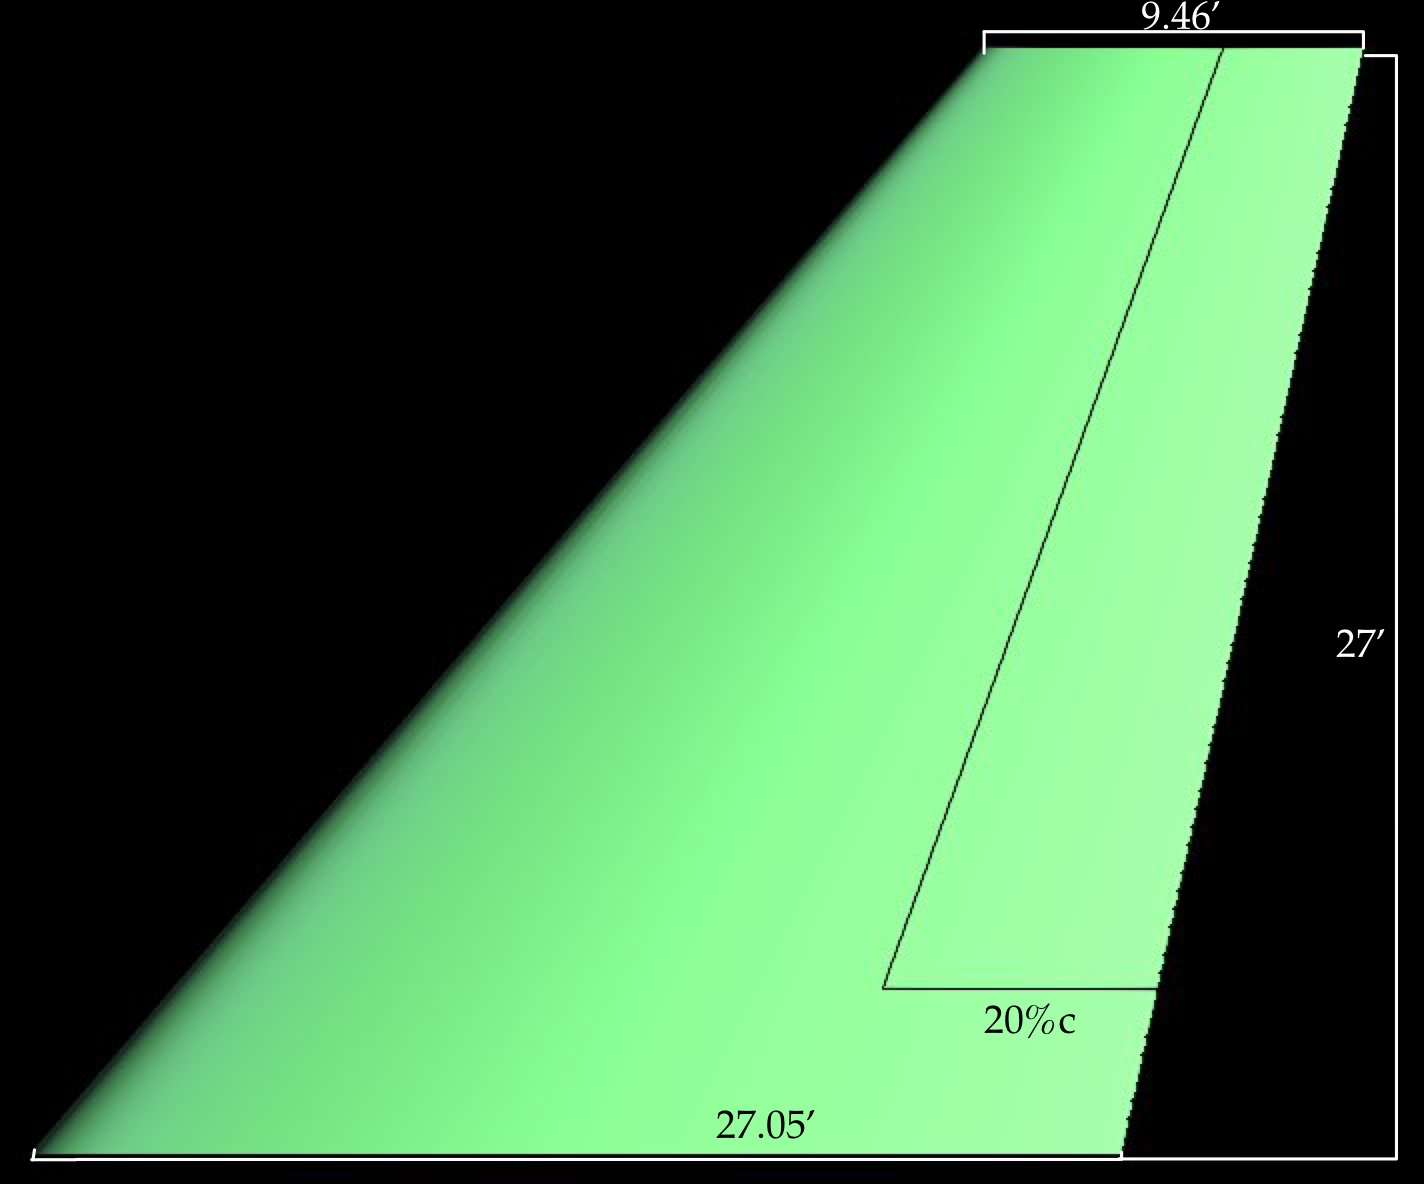
\includegraphics[width=0.65\textwidth]{Photos/stab/vtail.jpg}
    \caption{Vertical Stabilizer Side View}
    \label{fig:vtailstab}
\end{figure}
\clearpage

\subsection{Control Surfaces}
Several control surfaces are built into the wing, horizontal stabilizer, and vertical stabilizer.  The main wing contains a flap mechanism from spanwise locations $11.5$ ft to $69.1$ ft and deflects a maximum of $\delta_F = 30\degree$.  An initial aileron sizing has determined potential placement from $72$ ft to $90$ ft and has a deflection angle of $\pm 15\degree$.  During cruise, the ailerons lock into $\delta_f = 0\degree$ and outboard flap mechanism unlocks and deploys as a flaperon system to mitigate controllability issues at transonic cruise stage.  A trade study was conducted to determine whether SAM Mk I should lock ailerons and implement flaperons for the transonic cruise stage and it was determined to be more efficient to use flaperon systems at higher speeds and ailerons at slower speeds.  The rudder is located on the vertical tail and spans the entire length of the tail, $27$ ft, as is normal in comparable aircraft.  The maximum deflection angle of the rudder is $\pm 15\degree$.  The elevators are located on the horizontal stabilizer and spans from $2$ ft to $65$ ft.  Yet another trade study is taking place to determine the selection of trim tabs or a trimmable horizontal stabilizer.

\subsection{Modeling and Simulation}
A combination of OpenVSP and Athena Vortex Lattice (AVL) software is used to model SAM Mk I.  The OpenVSP model (Figure \ref{fig:simA}) provided a stepping stone in visualizing a preform of the aircraft during preliminary design stages.  OpenVSP was soon combined with AVL (Figure \ref{fig:simB}) to provide another blackbox procedure to simulating the controlability matrix. 

\begin{figure}[!h]
    \centering
    \begin{subfigure}{0.85\textwidth}
        \centering
        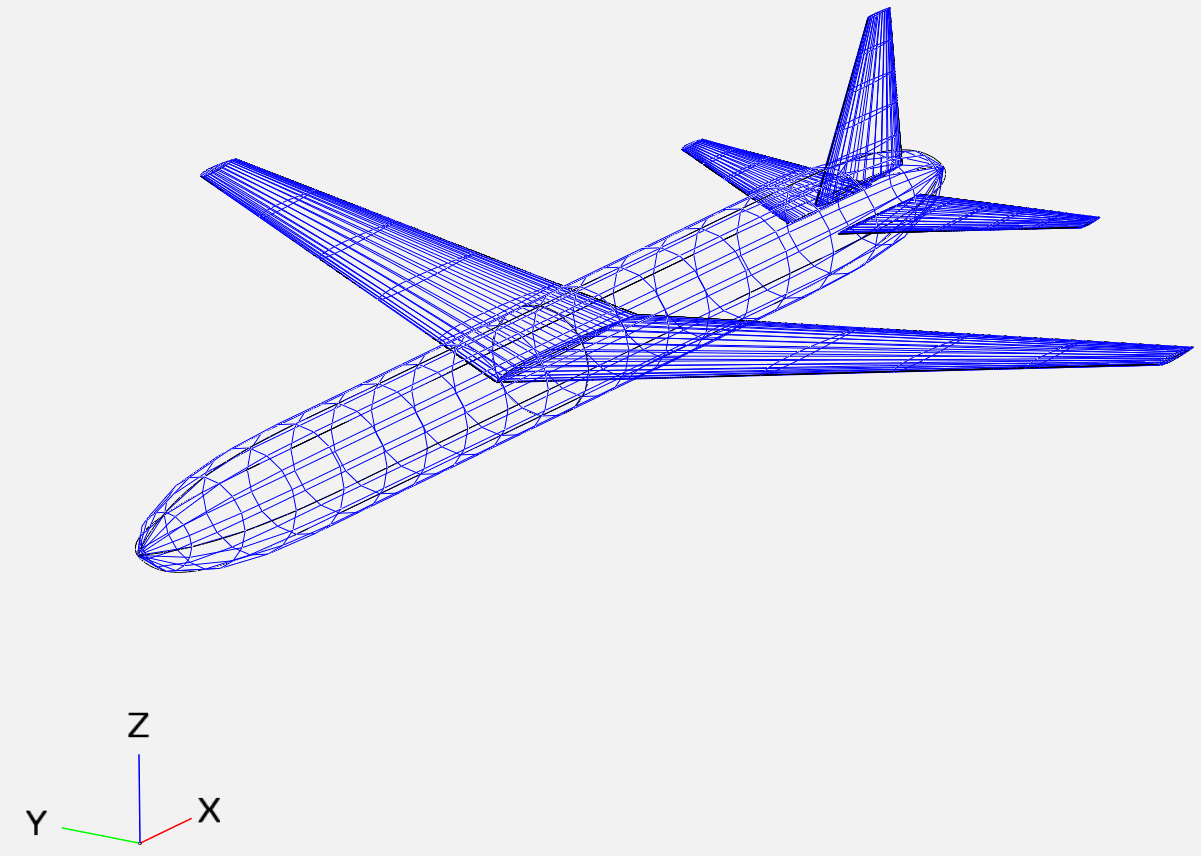
\includegraphics[width=\textwidth]{Photos/stab/openvsp.png}
        \caption{OpenVSP Model}
        \label{fig:simA}
    \end{subfigure}
    \begin{subfigure}{0.85\textwidth}
        \centering
        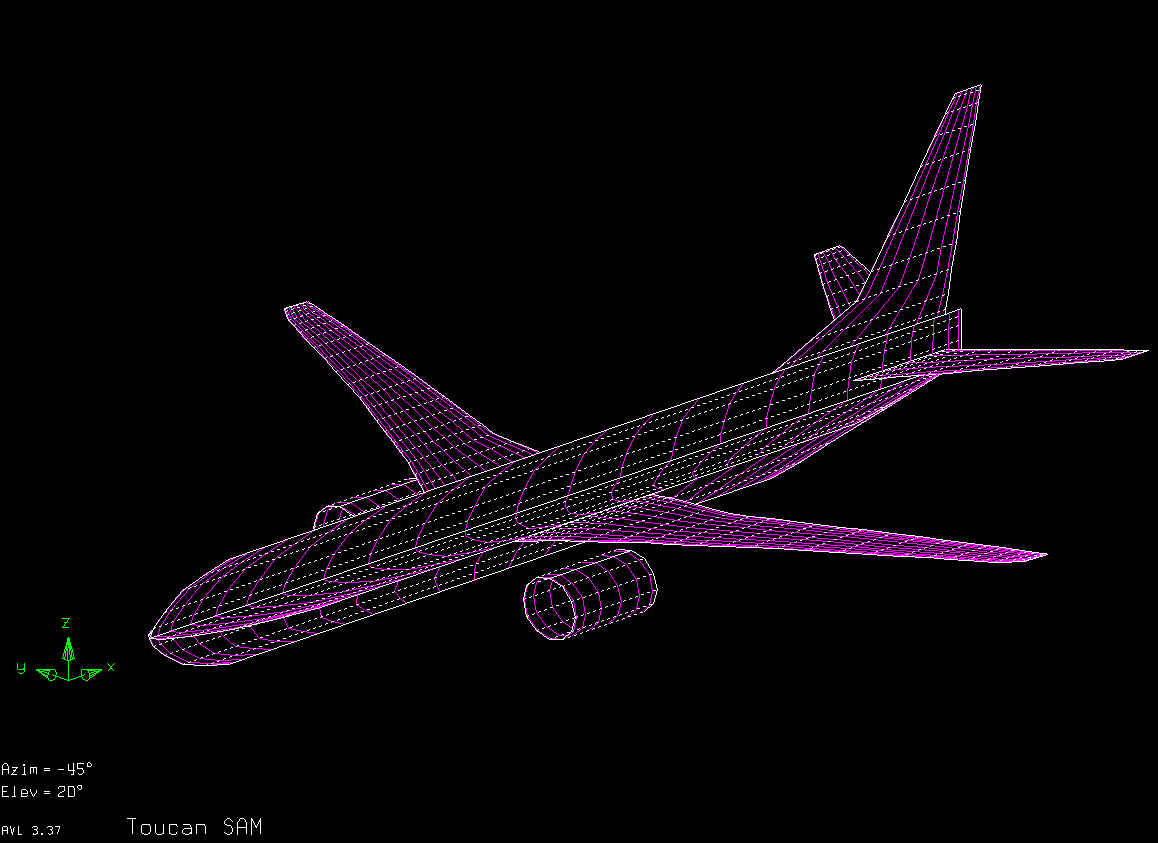
\includegraphics[width=\textwidth]{Photos/stab/avl.png}
        \caption{AVL Simulation}
        \label{fig:simB}
    \end{subfigure}
    \caption{Stability Simulations}
    \label{fig:sim}
\end{figure}
\clearpage

\subsection{Stability Control Derivatives}
Using Athena Vortex Lattice \cite{avl}, the following values in Table \ref{tab:deriv} were found using SAM Mk I dimensions.  The AVL stability derivatives function calculated $\frac{C_{l,\beta}C_{n,r}}{C_{l,r}C_{n,\beta}} = 2.214$, the value of which is greater than 1; therefore SAM Mk I has spiral stability.
\begin{table}[!h]
    \centering
    \caption{Stability Derivatives}
    \begin{tabular}{|c|c|}\toprule
        \textbf{Stability Derivative} & \textbf{Numerical Value} \\\hline\hline
        $C_{L,\alpha}$ & $1.91$ \\\hline
        $C_{m,\alpha}$ & $-1.25$ \\\hline
        $C_{l,\beta}$ & $-0.043$ \\\hline
        $C_{n,\beta}$ & $0.047$ \\\hline
        $C_{l,r}$ & $0.023$ \\\hline
        $C_{n,r}$ & $-0.058$ \\\hline
    \end{tabular}
    \label{tab:deriv}
\end{table}

\subsection{Longitudinal Static Stability}
AVL estimates the neutral point for this given aircraft to be approximately $X_{np} = 67.180$ ft aft of the nosecone.  Comparing AVL and OpenVSP, the value was found by simulation methods.
\begin{table}[!h]
    \centering
    \caption{Static Margin and Neutral Point}
    \begin{tabular}{|c||c|c|} \toprule
        \textbf{Criteria} & \textbf{Position [ft]} & \textbf{Position [Wing \% MAC]} \\\hline\hline
        $X_{CG}$ & 10.16 & 39.84 \\\hline
        $X_{NP}$ & 67.18 & 24.24\\\hline
        SM & 3.978 & 15.60 \\\bottomrule
    \end{tabular}
    \label{tab:statstab}
\end{table}
\clearpage
\subsection{Directional Stability}
SAM Mk I is equipped with rudder trim which enables the pilot and autopilot system to trim the control surface in the yaw direction to maintain stable flight in the case of a crosswind or in a take-off OEI situation.
\begin{figure}[!h]
    \centering
    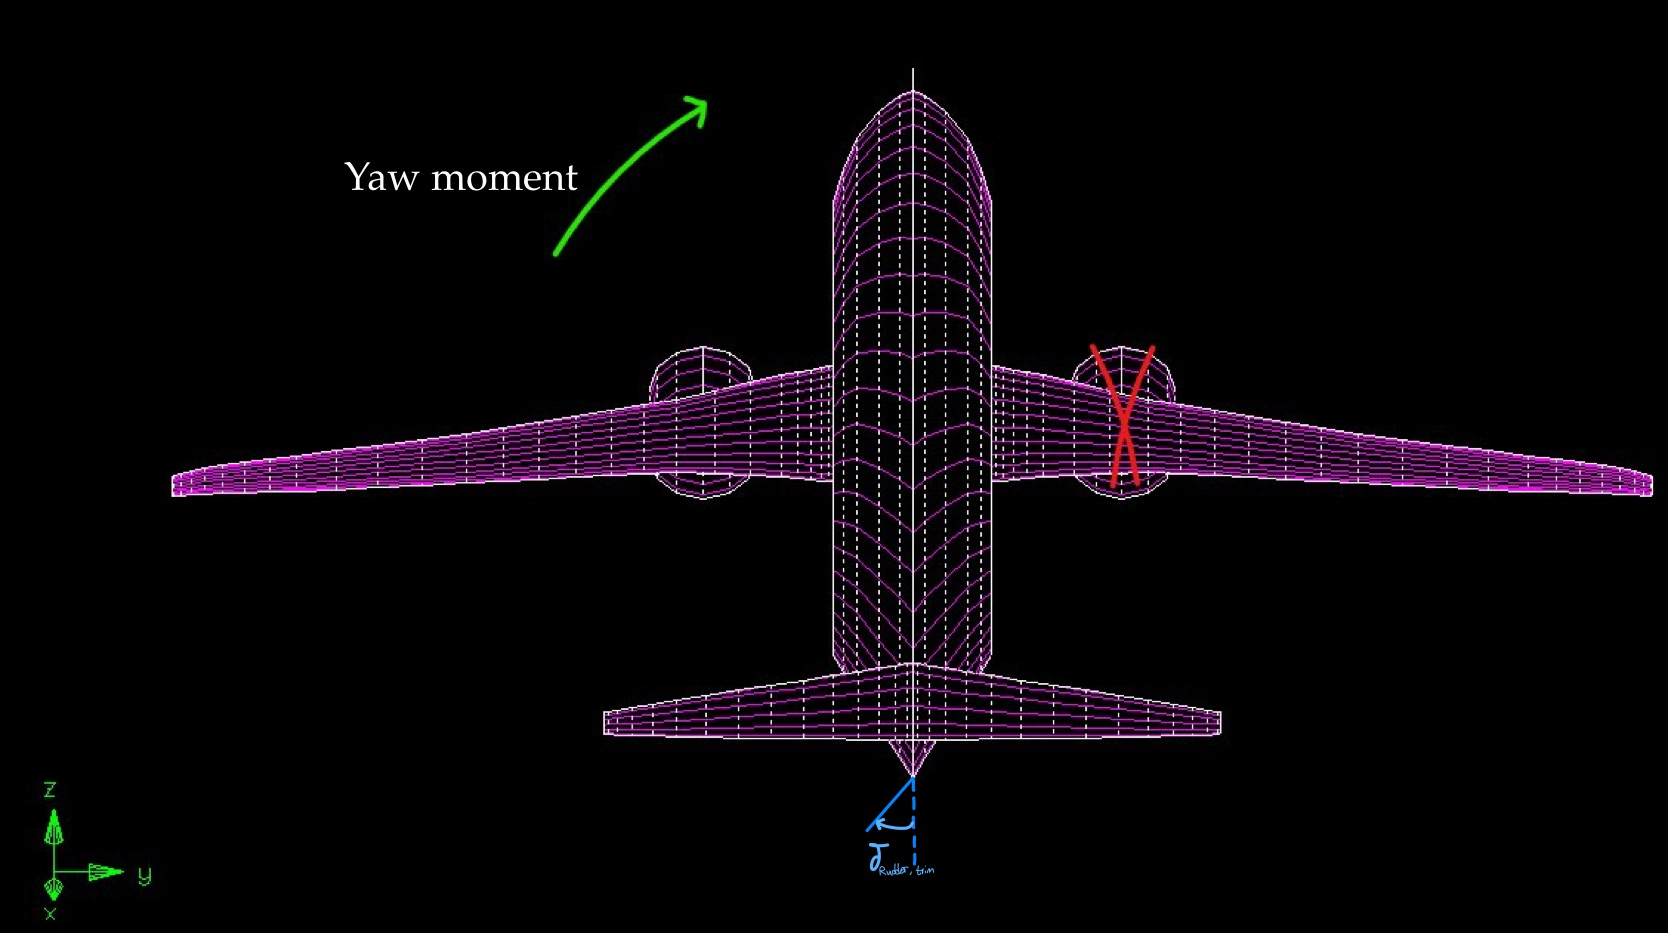
\includegraphics[width=\textwidth]{Photos/stab/oei.jpg}
    \caption{OEI Rudder Trim Simulation}
    \label{fig:OEI}
\end{figure}

% \subsection{Pitch Trim Control}


% \textcolor{red}{
% \begin{itemize}
%         \item Notch/scissor diagram (not required for PDR but will be for FDR)
%     \item Include incidence values for both the wing and horizontal stabilizer, with reasoning.
%     \item Provide trim diagrams with established trim points and elevator/stabilizer deflections.
%     \begin{itemize}
%         \item Have separate diagrams for takeoff, cruise, and landing.
%         \item Plot lines for at least 3 different elevator deflections (with indications in key).
%         \item Mark each trim point on its respective diagram.
%         \item Indicate takeoff, cruise, and landing deflections as interpolated, with $C_L$ values.
%     \end{itemize}
%     \item Discuss longitudinal static stability.
%     \begin{itemize}
%         \item Indicate static margin range and fore and aft CG locations used to find range.
%         \item Indicate neutral point location with calculation method.
%     \end{itemize}
%     \item Provide a list of stability control derivatives used in all calculations, with methodologies.
%     \begin{itemize}
%         \item Include (at minimum): $C_{L,\alpha}, C_{m,\alpha}, C_{m,\delta e},\varepsilon_{\alpha}$
%     \end{itemize}
%     \item Include at least two trade studies that use quantitative analysis to support design decisions made.
%     \item Discuss parachute incorporation if required.
%     \item Discuss future work.
%     \item \hl{AIAA: Summary of basic stability and control characteristics; this should include, but is not limited to static margin, pitch, roll and yaw derivatives}
% \end{itemize}}